% настройки в preamble.inc
\documentclass[14pt]{extarticle}

\usepackage[russian]{babel}
\usepackage[utf8]{inputenc}
\usepackage[T2A]{fontenc}

\usepackage{graphicx}  
\usepackage{amsfonts}
\usepackage{amsmath}
\usepackage{amssymb}
\usepackage{mathtools}
\usepackage{upgreek}
\usepackage{xfrac}


\usepackage{listings}

\lstset{
	captionpos=t,
	breaklines=true,         % автоматически переносить строки 
	breakatwhitespace=false, % переносить строки по пробелу
	%backgroundcolor=\color{mylightgray},rulecolor=\color{red},  % choose the background color; you must add \usepackage{color} or \usepackage{xcolor}; should come as last argument
	basicstyle=\footnotesize\ttfamily,        % the size of the fonts that are used for the code
	breakatwhitespace=false,         % sets if automatic breaks should only happen at whitespace
	breaklines=true,                 % sets automatic line breaking
	captionpos=t,                    % sets the caption-position to bottom
	commentstyle=\color{green},    % comment style
	extendedchars=false,              % lets you use non-ASCII characters; for 8-bits encodings only, does not work with UTF-8
	firstnumber=0,                % start line enumeration with line 1000
	frame=single,
	%rulesepcolor=\color{green},	                   % adds a frame around the code
	keepspaces=true,                 % keeps spaces in text, useful for keeping indentation of code (possibly needs columns=flexible)
	keywordstyle=\color{blue}\textbf,       % keyword style
	language=python,                 % the language of the code
	morekeywords={*,...},            % if you want to add more keywords to the set
	numbers=left,                    % where to put the line-numbers; possible values are (none, left, right)
	numbersep=5pt,                   % how far the line-numbers are from the code
	%numberstyle=\scriptsize\color{mygray}, % the style that is used for the line-numbers
	rulecolor=\color{black},         % if not set, the frame-color may be changed on line-breaks within not-black text (e.g. comments (green here))
	showspaces=false,                % show spaces everywhere adding particular underscores; it overrides 'showstringspaces'
	showstringspaces=false,          % underline spaces within strings only
	showtabs=false,                  % show tabs within strings adding particular underscores
	stepnumber=1,                    % the step between two line-numbers. If it's 1, each line will be numbered
	%stringstyle=\color{mymauve},     % string literal style
	tabsize=4,	                   % sets default tabsize to 2 spaces
	%title=\lstname                   % show the filename of files included with \lstinputlisting; also try caption instead of title
}

\lstset{
	captionpos=t,
	breaklines=true,         % автоматически переносить строки 
	breakatwhitespace=false, % переносить строки по пробелу
	%backgroundcolor=\color{mylightgray},rulecolor=\color{red},  % choose the background color; you must add \usepackage{color} or \usepackage{xcolor}; should come as last argument
	basicstyle=\footnotesize\ttfamily,        % the size of the fonts that are used for the code
	breakatwhitespace=false,         % sets if automatic breaks should only happen at whitespace
	breaklines=true,                 % sets automatic line breaking
	captionpos=t,                    % sets the caption-position to bottom
	commentstyle=\color{green},    % comment style
	extendedchars=false,              % lets you use non-ASCII characters; for 8-bits encodings only, does not work with UTF-8
	firstnumber=0,                % start line enumeration with line 1000
	frame=single,
	%rulesepcolor=\color{green},	                   % adds a frame around the code
	keepspaces=true,                 % keeps spaces in text, useful for keeping indentation of code (possibly needs columns=flexible)
	keywordstyle=\color{blue}\textbf,       % keyword style
	language=SQL,                 % the language of the code
	morekeywords={*,...},            % if you want to add more keywords to the set
	numbers=left,                    % where to put the line-numbers; possible values are (none, left, right)
	numbersep=5pt,                   % how far the line-numbers are from the code
	%numberstyle=\scriptsize\color{mygray}, % the style that is used for the line-numbers
	rulecolor=\color{black},         % if not set, the frame-color may be changed on line-breaks within not-black text (e.g. comments (green here))
	showspaces=false,                % show spaces everywhere adding particular underscores; it overrides 'showstringspaces'
	showstringspaces=false,          % underline spaces within strings only
	showtabs=false,                  % show tabs within strings adding particular underscores
	stepnumber=1,                    % the step between two line-numbers. If it's 1, each line will be numbered
	%stringstyle=\color{mymauve},     % string literal style
	tabsize=4,	                   % sets default tabsize to 2 spaces
	%title=\lstname                   % show the filename of files included with \lstinputlisting; also try caption instead of title
}

\usepackage{enumerate}
%\usepackage{multirow}
%\usepackage{tikz}
%\usetikzlibrary{arrows,positioning,shadows}
%\usepackage{paralist,array}

\usepackage{geometry}
\geometry{right=20mm}
\geometry{left=30mm}
\geometry{bottom=20mm}
\geometry{ignorefoot}% считать от нижней границы текста

\setlength{\parindent}{1.25 cm}
\setlength{\parskip}{1ex}
\renewcommand{\baselinestretch}{1.5}

\usepackage[toc,page]{appendix}

\usepackage{titlesec}
\titleformat{\section}
  {\normalfont\fontsize{14}{14}\bfseries}{\thesection}{1em}{}
\titleformat{\subsection}
  {\normalfont\fontsize{14}{14}\bfseries}{\thesubsection}{1em}{}

\usepackage[intoc]{nomencl}
\renewcommand{\nomname}{Обозначения и сокращения}
\makenomenclature

%Подписи
\usepackage		[margin		= 10	pt,
%					font		= footnotesize, 
					labelfont	= bf, 
					labelsep	= endash, 
					labelfont	= bf,
%					textfont	= sl,
					margin		= 0 	pt,  
					aboveskip 	= 4		pt, 
					belowskip 	= -6	pt,
					figurename= Рисунок] {caption}
\usepackage		[margin		= 10	pt,
					font		= footnotesize, 
					labelfont	= bf, 
					labelsep	= endash, 
					labelfont	= bf,
					textfont	= sl,
					margin		= 0 	pt,  
					aboveskip 	= 4		pt, 
					belowskip 	= 6	pt]	{subcaption}


\newcommand\Referat{%реферат
	\chapter*{Реферат}%
}

\addto\captionsrussian{%
	\def\contentsname{%
		Содержание}%
	\def\bibname{%
		Список~
		использованных~
		источников}%
}


\usepackage{enumitem}
\usepackage{kosrem}
\usepackage{gensymb}


\begin{document}




\setcounter{page}{3}

% СОДЕРЖАНИЕ 
\clearpage
\tableofcontents

% ВВЕДЕНИЕ
\clearpage
\section*{Введение}
\addcontentsline{toc}{section}{Введение}
В современном мире регулирование широко используемых в профессиональном спорте трансферов (переходов) спортсменов — это тема, к которой спортивная общественность, СМИ и государство проявляют обоснованный интерес. На протяжении последнего столетия регламентными нормами неправительственных спортивных организаций сформирован особый механизм смены спортсменами своих работодателей. Ясно, что эти особенности наиболее ярко проявляются в самых популярных и массовых командных видах спорта — футболе, хоккее, баскетболе и т. д. Очевидно, что организациям необходимы удобные приложения для проведения сделок по покупке и продаже игроков.

Целью данной работы является реализация простого в использовании и многофункционального приложения для получения информации об игроках с возможностью их покупки и продажи.

Для достижения поставленной цели необходимо решить следующие задачи:
\begin{itemize}
	\item[1)] формализовать задание, выделив соответствующих пользователей и их функционал;
	\item[2)] провести анализ СУБД и выбрать наиболее подходящую;
	\item[3)] спроектировать базу данных;
	\item[4)] спроектировать архитектуру приложения;
	\item[5)] разработать приложение.
\end{itemize}

% АНАЛИТИЧЕСКАЯ ЧАСТЬ
\clearpage
\section{Аналитический раздел}
В данном разделе будет поставлена задача, рассмотрены возможные пользователи системы, модели данных и СУБД.

\subsection{Постановка задачи}
Необходимо разработать программу, предоставляющую интерфейс для получения информации об игроках по заданным параметрами с возможностью их покупки и продажи.
\subsection{Пользователи системы}
\subsubsection{Гость}
Гость — это неавторизованный пользователь, обладающий только одной возможностью взаимодействия с системой - авторизация.
\subsubsection{Аналитик}
Аналитик - это авторизированный пользователь, закрепленный за определенной командой, обладающий базовыми возможностями взаимодействия с системой - просмотр информации об игроках, их статистике за прошедший сезон и командах. Также дополнительными возможностями аналитика являются просмотр желаемых игроков для своей команды, добавление игрока в список желаемых игроков команды и удаление желаемого игрока из этого списка.
\subsubsection{Менеджер} 
Менеджер - это авторизованный пользователь, закрпеленный за определенной, обладающий базовыми возможностями взаимодействия с системой - просмотр информации об игроках, их статистике за прошедший сезон и командах. Также дополнительными возможностями менеджера являются просмотр желаемых игроков для своей команды, удаление желаемого игрока из списка желаемых игроков. Менеджер может запрашивать игрока у другой команды, подтверждать и отклонять доступные сделки.
\subsubsection{Модератор}
Модератор является авторизированным пользователем с повышенным уровнем полномочий — он обладает всеми базовыми правами пользователя, а также может проводить и удалять сделки, изменять баланс команды и команду игрока.
\subsection{Анализ моделей баз данных}
Модель базы данных - это тип модели данных, которая определяет логическую структуру базы данных и в корне определяет, каким образом данные могут храниться, организовываться и обрабатываться.

\subsubsection{Иерархическая база данных}
Иерархическая модель базы данных подразумевает, что элементы организованы в структуры, связанные между собой иерархическими или древовидными связями. Родительский элемент может иметь несколько дочерних элементов. Но у дочернего элемента может быть только один предок.

Иерархические базы данных графически могут быть представлены как перевернутое дерево, состоящее из объектов различных уровней. Верхний уровень (корень дерева) занимает один объект, второй - объекты второго уровня и так далее. 

Такая модель подразумевает возможность существования одинаковых (преимущественно дочерних) элементов. Данные здесь хранятся в серии записей с прикреплёнными к ним полями значений. Модель собирает вместе все экземпляры определённой записи в виде «типов записей» — они эквивалентны таблицам в реляционной модели, а отдельные записи — столбцам таблицы.

\subsubsection{Сетевая модель базы данных}
Сетевая модель базы данных подразумевает, что у родительского элемента может быть несколько потомков, а у дочернего элемента — несколько предков. Записи в такой модели связаны списками с указателями. 

Сетевая модель состоит из множества записей, которые могут быть владельцами или членами групповых отношений. Связь между записью-владельцем и записью-членом также имеет вид 1:N.

Сетевая модель позволяет иметь несколько предков и потомков, формирующих решётчатую структуру.

На рисунке \ref{img:set} представлен пример сетевой модели базы данных.

\begin{figure}[h!]
	\centering
	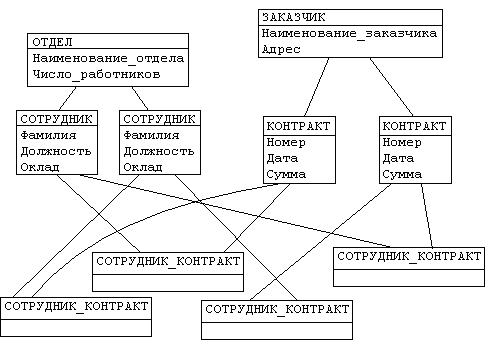
\includegraphics[scale=1]{img/set.png}
	\caption{Иерархическая модель базы данных}
	\label{img:set}
\end{figure}

\subsubsection{Реляционная модель базы данных}
В реляционной модели, в отличие от иерархической или сетевой, не существует физических отношений. Вся информация хранится в виде таблиц (отношений), состоящих из рядов и столбцов. А данные двух таблиц связаны общими столбцами, а не физическими ссылками или указателями. Для манипуляций с рядами данных существуют специальные операторы.

Реляционные таблицы обладают следующими свойствами:
\begin{itemize}
	\item[1)] все значения атомарны;
	\item[2)] каждый ряд уникален;
	\item[3)] порядок столбцов не важен;
	\item[4)] порядок рядов не важен;
	\item[5)] у каждого столбца есть своё уникальное имя.
\end{itemize}

Термин «реляционный» означает, что теория основана на математическом понятии отношение (relation). В качестве неформального синонима термину «отношение» часто встречается слово таблица. Необходимо помнить, что «таблица» есть понятие нестрогое и неформальное и часто означает не «отношение» как абстрактное понятие, а визуальное представление отношения на бумаге или экране. Некорректное и нестрогое использование термина «таблица» вместо термина «отношение» нередко приводит к недопониманию.

\subsubsection{Выбор модели данных}
В качестве модели данных была выбрана реляционная модель, так как структура данных однозначно определена, структура данных не является быстроизменяющейся и данные подчиняются строгим правилам и ограничениям.

\subsection{Вывод}
В данном разделе была поставлена задача, рассмотрены возможные пользователи системы, проанализированы модели данных и СУБД.


%КОНСТРУКТОРСКИЙ РАЗДЕЛ
\clearpage
\section{Конструкторский раздел}
В данном разделе будут рассотрены сценарии пользователей, спроектирована база данных, описана ролевая модель и спроектировано приложение.
\subsection{Сценарии пользователей}
Необходимо определить функционал каждого из пользователей. 
\subsubsection{Гость}
Гость - это неавторизованный пользователь, у которого есть только одна возможность - авторизоваться. На рисунке \ref{img:UseCaseGuest} представлена Use-Case-диаграмма для гостя.

\begin{figure}[h!]
	\centering
	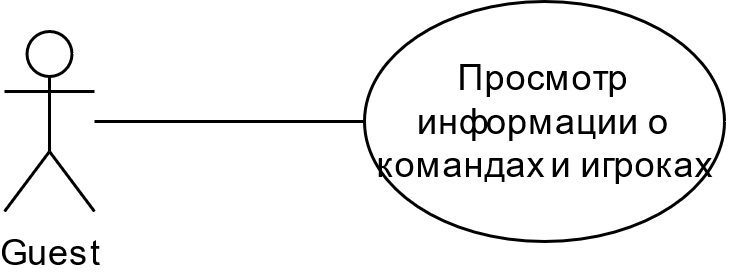
\includegraphics[scale=0.35]{img/UseCaseGuest.png}
	\caption{Сценарии для гостя.}
	\label{img:UseCaseGuest}
\end{figure}

\subsubsection{Любой авторизированный пользователь}
Функциональность, предоставляемая каждому авторизированного пользователя (аналитику, менеджеру, модератору):
\begin{itemize}
	\item[1)] просмотр всех игроков;
	\item[2)] просмотр статистики игроков;
	\item[3)] получение игроков выбранной команды;
	\item[4)] поиск игрока по ID;
	\item[5)] поиск игрока по имени;
	\item[6)] просмотр всех команд;
	\item[7)] поиск команды по ID;
	\item[8)] поиск команды по имени;
	\item[9)] получение статистики выбранного игрока.      
\end{itemize}
\subsubsection{Аналитик}
Дополнительная функциональность, предоставляемая пользователю аналитик:
\begin{itemize}
	\item[1)] добавить желаемого игрока;
	\item[2)] удалить желаемого игрока;
	\item[3)] просмотр всех желаемых игроков.  
\end{itemize}
На рисунке \ref{img:UseCaseAnalytic} представлена Use-Case-диаграмма для аналитика.
\begin{figure}[h!]
	\centering
	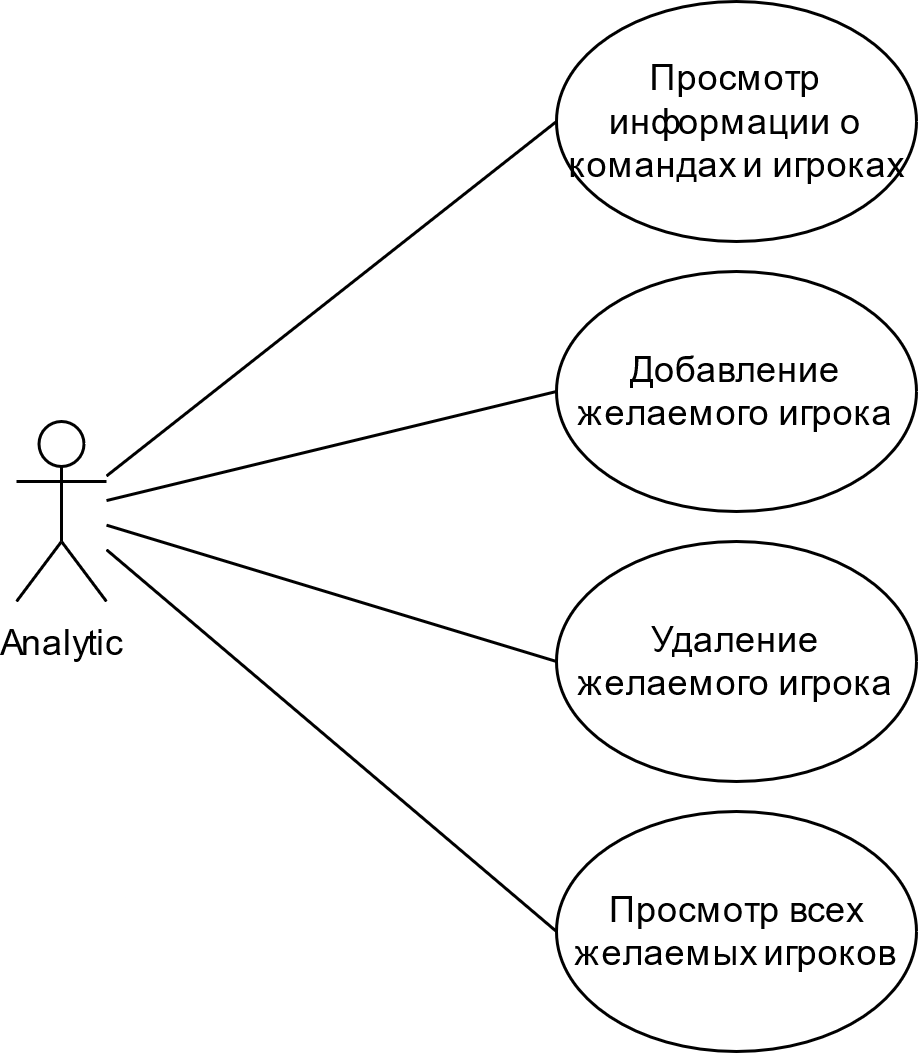
\includegraphics[scale=0.35]{img/UseCaseAnalytic.png}
	\caption{Сценарии для аналитика.}
	\label{img:UseCaseAnalytic}
\end{figure}
\subsubsection{Менеджер}
Дополнительная функциональность, предоставляемая пользователю менеджер:
\begin{itemize}
	\item[1)] просмотр всех желаемых игроков;
	\item[2)] удалить желаемого игрока; 
	\item[3)] запросить желаемого игрока с указанием предлагаемой цены;
	\item[4)] подтвердить сделку;
	\item[5)] отклонить сделку;
	\item[6)] получить входящие предложения;
	\item[7)] получить исходящие предложения.    
\end{itemize}
На рисунке \ref{img:UseCaseManager} представлена Use-Case-диаграмма для менеджера.
\begin{figure}[h!]
	\centering
	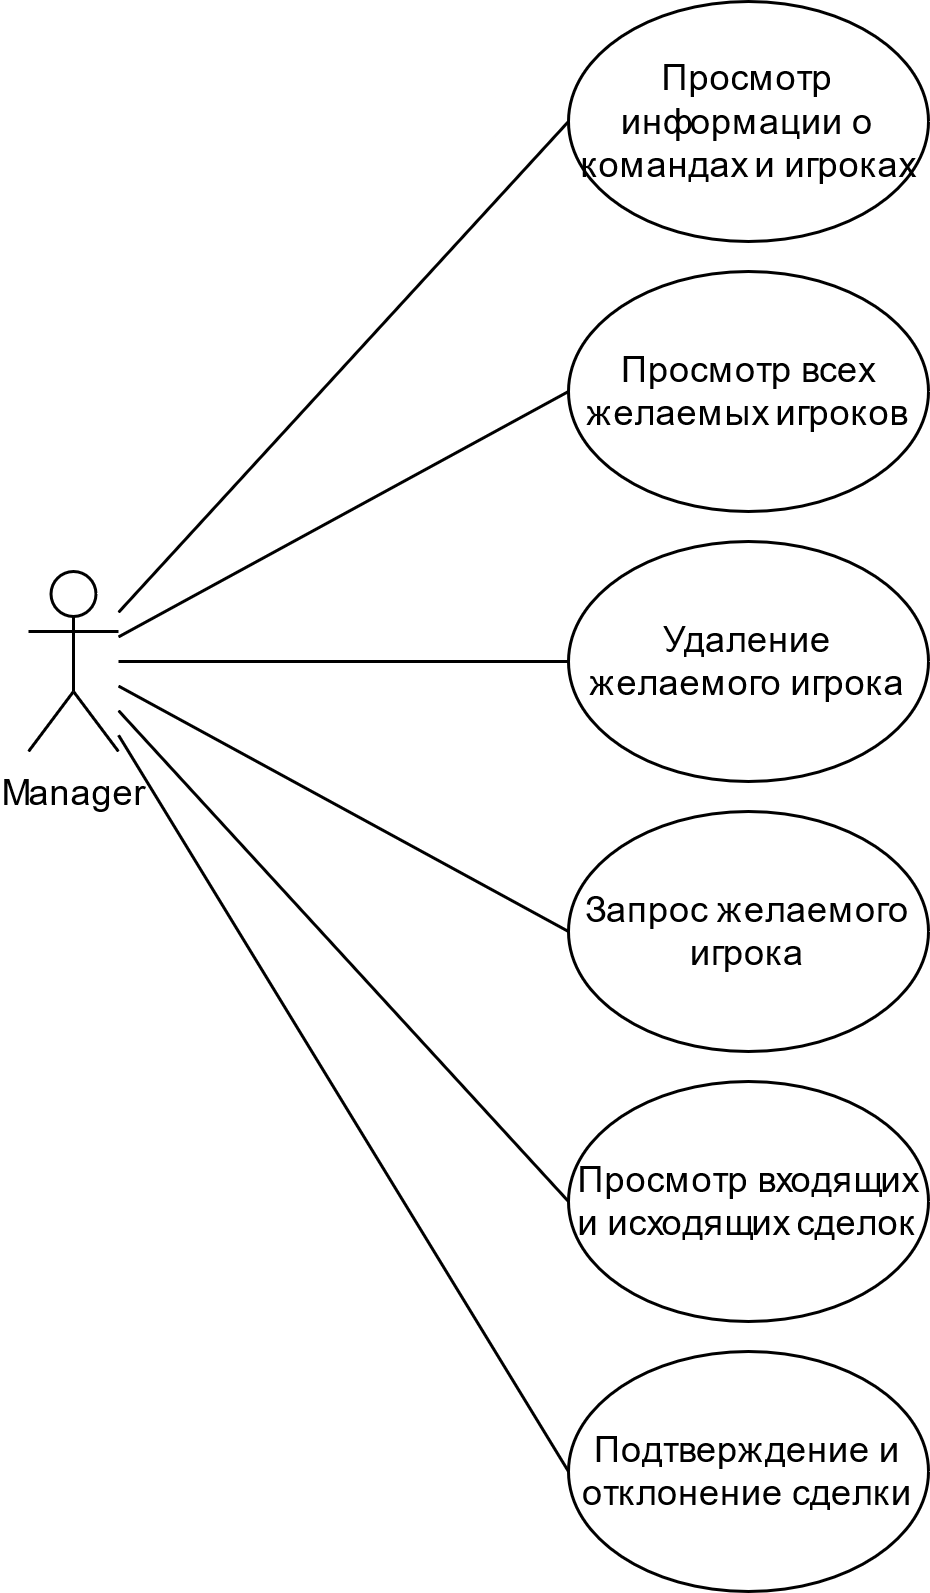
\includegraphics[scale=0.25]{img/UseCaseManager.png}
	\caption{Сценарии для менеджера.}
	\label{img:UseCaseManager}
\end{figure}
\subsubsection{Модератор}
Дополнительная функциональность, предоставляемая пользователю модератор:
\begin{itemize}
	\item[1)] провести сделку;
	\item[2)] удалить сделку;
	\item[3)] изменить команду игрока;
	\item[4)] изменить баланс команды;
	\item[5)] просмотр всех пользователей;
	\item[6)] добавление нового пользователя;
	\item[7)] удаление пользователя.  
\end{itemize}
На рисунке \ref{img:UseCaseModerator} представлена Use-Case-диаграмма для модератора.
\begin{figure}[h!]
	\centering
	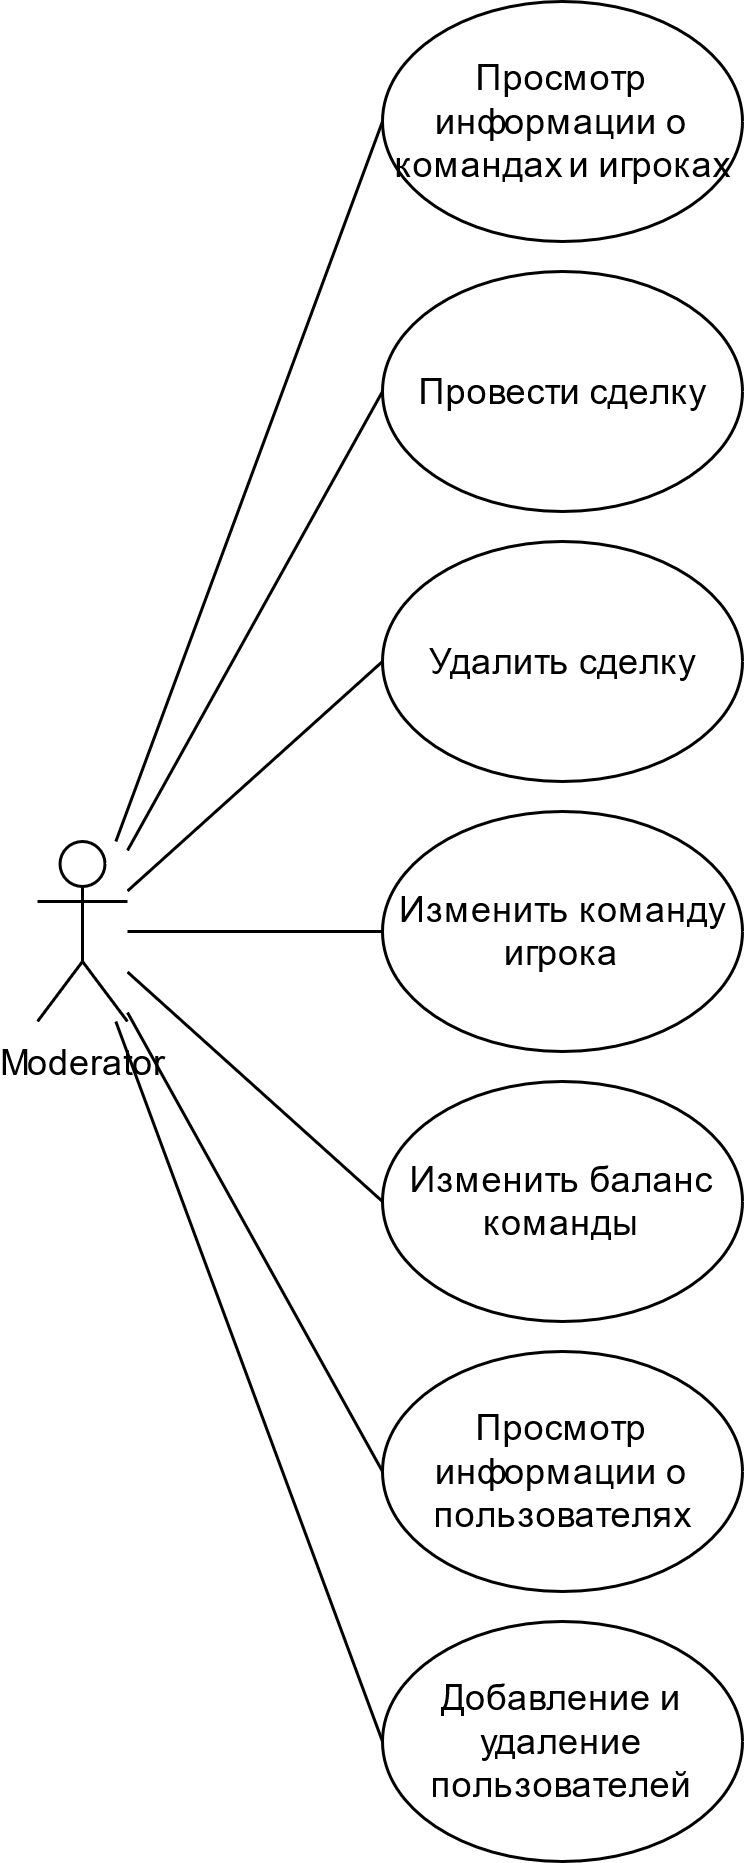
\includegraphics[scale=0.25]{img/UseCaseModerator.png}
	\caption{Сценарии для модератора.}
	\label{img:UseCaseModerator}
\end{figure}
\newpage

\subsection{Проектирование базы данных}
\subsubsection{Формализация сущностей системы}
Необходимо выделить сущности предметной области и построить ER-диаграмму. 
На рисунке \ref{img:ER} представлена ER-диаграмма системы.
\begin{figure}[h!]
	\centering
	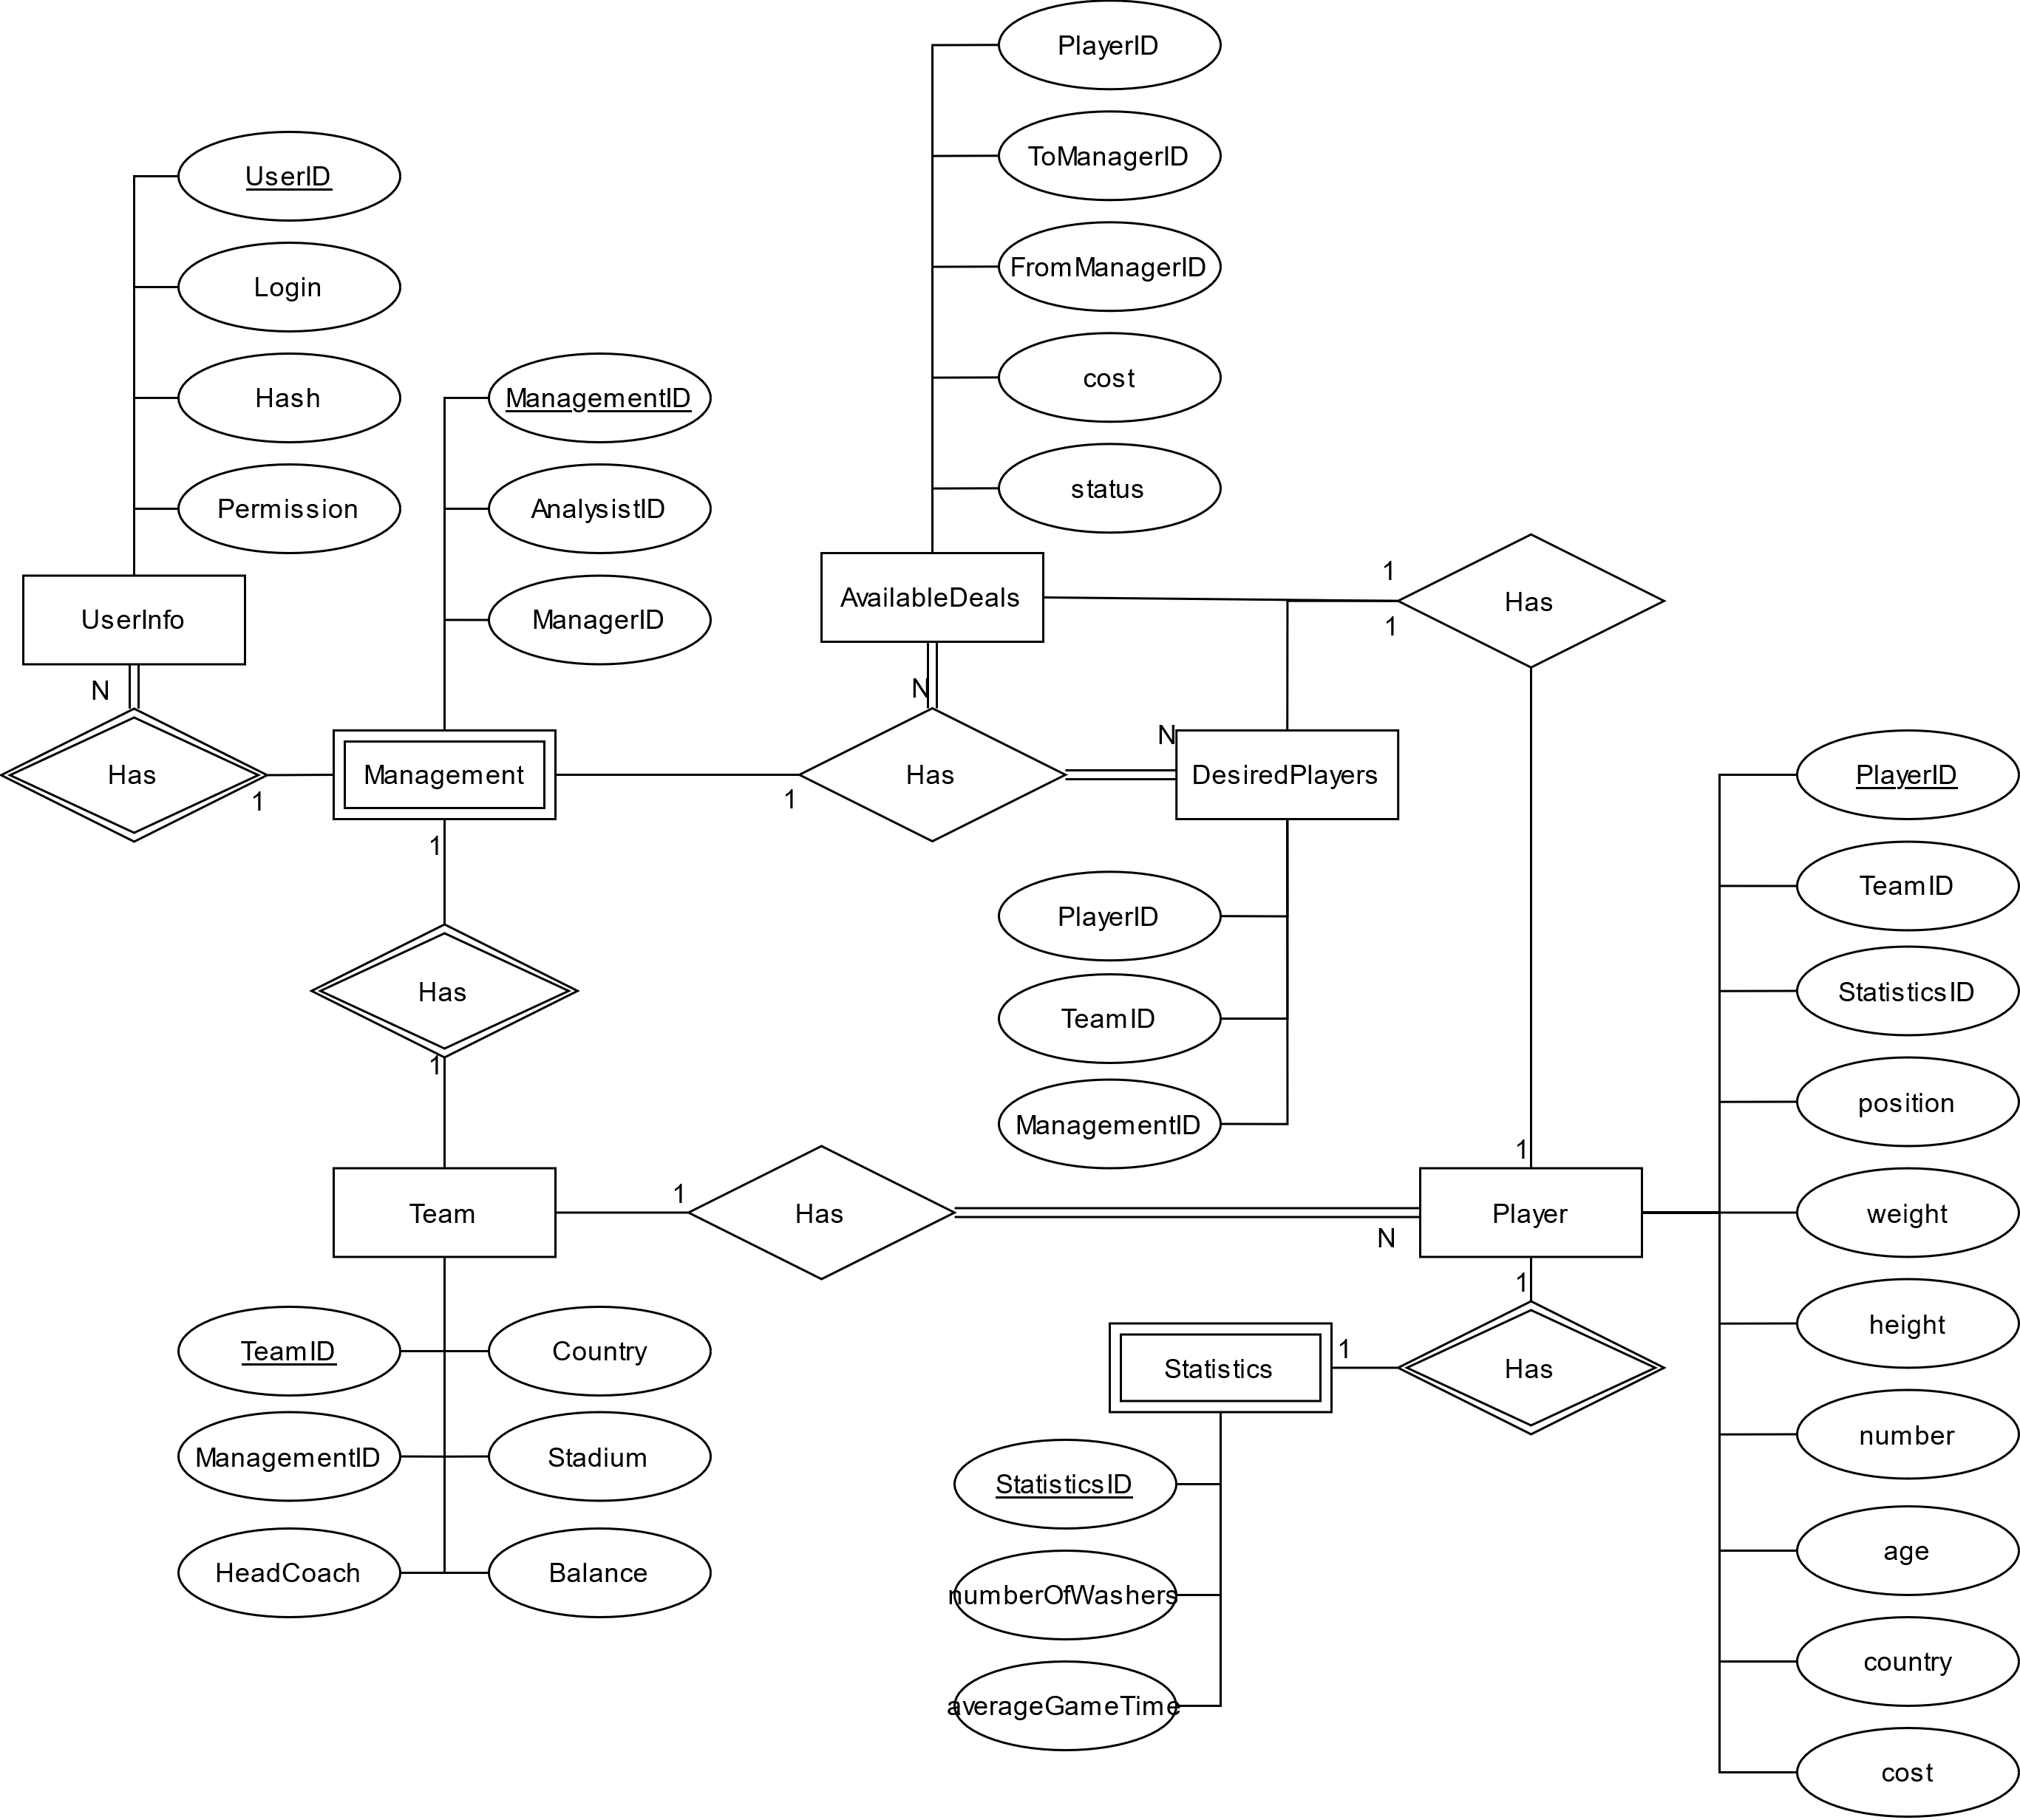
\includegraphics[scale=0.18]{img/ER.png}
	\caption{ER-диаграмма системы.}
	\label{img:ER}
\end{figure}
\newpage
Выделенные сущности:
\begin{itemize}
	\item[1)] UserInfo - таблица, в которой хранится информация о пользователях;
	\item[2)] Management - таблица, в которой хранятся ID аналитиков и менеджеров, которые закреплены за определенной командой;
	\item[3)] Team - таблица, в которой хранится информация о командах;
	\item[4)] Player - таблица, в которой хранится информация об игроках;
	\item[5)] AvailableDeals - таблица, в которой хранится информация о доступных сделках определенного менеджмента;
	\item[6)] DesiredPlayers - таблица, в которой хранится информация о желаемых игроках определенного менеджмента;
	\item[7)] Statistics - таблица, в которой хранится информация о статистике определенного игрока.
\end{itemize}

\subsubsection{Ролевая модель}
На уровне базы данных выделена следующая ролевая модель:
\begin{itemize}
	\item[1)] guest - гость;
	\item[2)] analytic - аналитик;
	\item[3)] manager - менеджер;
	\item[4)] moderator - модератор.  
\end{itemize}
Использование ролевой модели на уровне базы данных гарантирует безопасность доступа к объектам базы данных.

\textbf{Гость}\\
Пользователь с ролью guest имеет следующие права: SELECT над таблицей UserInfo.

\textbf{Аналитик}\\
Пользователь с ролью analytic имеет следующие права:
\begin{itemize}
	\item[1)] SELECT над таблицей Player;
	\item[2)] SELECT над таблицей Management; 
	\item[3)] SELECT над таблицей Team;
	\item[4)] SELECT над таблицей Statistics;
	\item[5)] SELECT, UPDATE, DELETE, INSERT над таблицей DesiredPlayers.    
\end{itemize}

\textbf{Менеджер}\\
Пользователь с ролью manager имеет следующие права:
\begin{itemize}
	\item[1)] SELECT над таблицей Player;
	\item[2)] SELECT над таблицей Management; 
	\item[3)] SELECT над таблицей Team;
	\item[4)] SELECT над таблицей Statistics;
	\item[5)] SELECT, DELETE над таблицей DesiredPlayers.    
	\item[6)] SELECT, DELETE, INSERT над таблицей AvailableDeals.
\end{itemize}
\textbf{Модератор}\\
Пользователь с ролью moderator обладает всеми правами.

\subsubsection{Функции}
Для того, чтобы пользователь мог одновременно просматривать информацию об игроке, его команде и его статистику, необходимо добавить функцию, которая возвращает эту информацию. На рисунке \ref{img:func} представлен алгоритм функции.

\begin{figure}[h!]
	\centering
	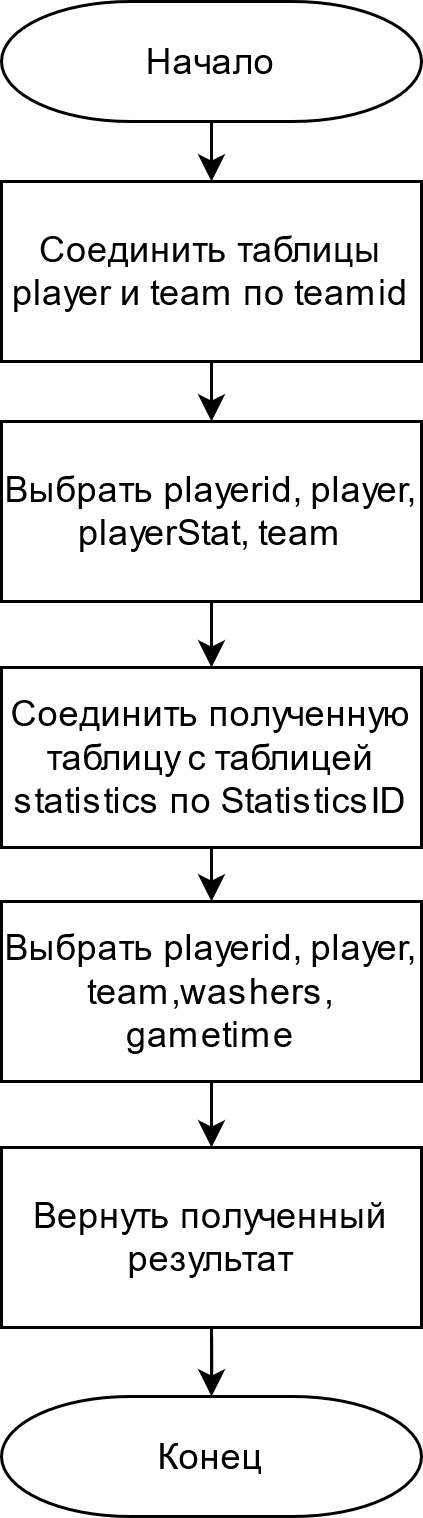
\includegraphics[scale=0.30]{img/func.png}
	\caption{Алгоритм функции.}
	\label{img:func}
\end{figure}
\newpage
\subsection{Проектирование приложения}
Приложение для работы с базой данных представляет собой Desktop-приложение. Оно спроектировано по паттерну MVC. Выделены два компонента - доступа к данным и бизнес-логики. Компонент доступа к данным спроектирован по паттерну "Репозиторий". Для контроля ролей при авторизации пользователя создан класс Connection, в котором обрабатывается конфигурационный файл и возвращается строка подключения. 
\subsection{Вывод}
В данном разделе были рассмотрены сценарии пользователей, спроектирована база данных, описана ролевая модель и спроектировано приложение.

\newpage
%ТЕХНОЛОГИЧЕСКИЙ РАЗДЕЛ
\section{Технологический раздел}
В данном разделе будут выбраны средства реализации поставленной задачи, создана база данных и ролевая модель, разработаны компоненты и описан порядок работы.
\subsection{Анализ СУБД}
СУБД — комплекс программ, позволяющих создать базу данных (БД) и манипулировать данными (вставлять, обновлять, удалять и выбирать). Система обеспечивает безопасность, надёжность хранения и целостность данных, а также предоставляет средства для администрирования БД. Самыми популярными СУБД являются MySQL, Microsoft SQL Server, PostgreSQL и Oracle.
\subsubsection{MySQL}
MySQL — реляционная СУБД с открытым исходным кодом, главными плюсами которой являются ее скорость и гибкость, которая обеспечена поддержкой большого количества различных типов таблиц.

Кроме того, это надежная бесплатная система с простым интерфейсом и возможностью синхронизации с другими базами данных. В совокупности эти факторы позволяют использовать MySQL как крупным корпорациям, так и небольшим компаниям.

Преимущества:
\begin{itemize}
	\item[1)] простота в использовании;
	\item[2)] обширный функционал;
	\item[3)] безопасность;
	\item[4)] масштабируемость;
	\item[5)] скорость.    
\end{itemize}
Недостатки: недостаточная надежность;
\subsubsection{Microsoft SQL Server}
Система позволяет синхронизироваться с другими программными продуктами компании Microsoft, а также обеспечивает надежную защиту данных и простой интерфейс, однако отличается высокой стоимостью лицензии и повышенным потреблением ресурсов.

Преимущества:
\begin{itemize}
	\item[1)] СУБД масштабируется;
	\item[2)] простота в использовании;
	\item[3)] возможность интеграции с другими продуктами Microsoft.  
\end{itemize}
Недостатки:
\begin{itemize}
	\item[1)] высокая стоимость продукта для юридических лиц; 
	\item[2)] возможны проблемы в работе служб интеграции импорта файлов;
	\item[3)] высокая ресурсоемкость SQL Server.  
\end{itemize}
\subsubsection{PostgreSQL}
PostgreSQL — это популярная свободная объектно-реляционная система управления базами данных. PostgreSQL базируется на языке SQL и поддерживает многочисленные возможности.

Преимущества:
\begin{itemize}
	\item[1)] бесплатное ПО с открытым исходным кодом;
	\item[2)] большое количество дополнений;
	\item[3)] расширения;   
\end{itemize}
Недостатки:
\begin{itemize}
	\item[1)] производительность;
	\item[2)] популярность;  
\end{itemize}
\subsubsection{Oracle}
Oracle – это объектно-реляционная система управления базами данных.

Преимущества:
\begin{itemize}
	\item[1)] поддержка огромных баз данных;
	\item[2)] быстрая обработка транзакций;
	\item[3)] большой и постоянно развивающийся функционал.   
\end{itemize}
Недостатки:
\begin{itemize}
	\item[1)] высокая стоимость; 
	\item[2)] значительные вычислительные ресурсы. 
\end{itemize}

\begin{figure}[h!]
	\centering
	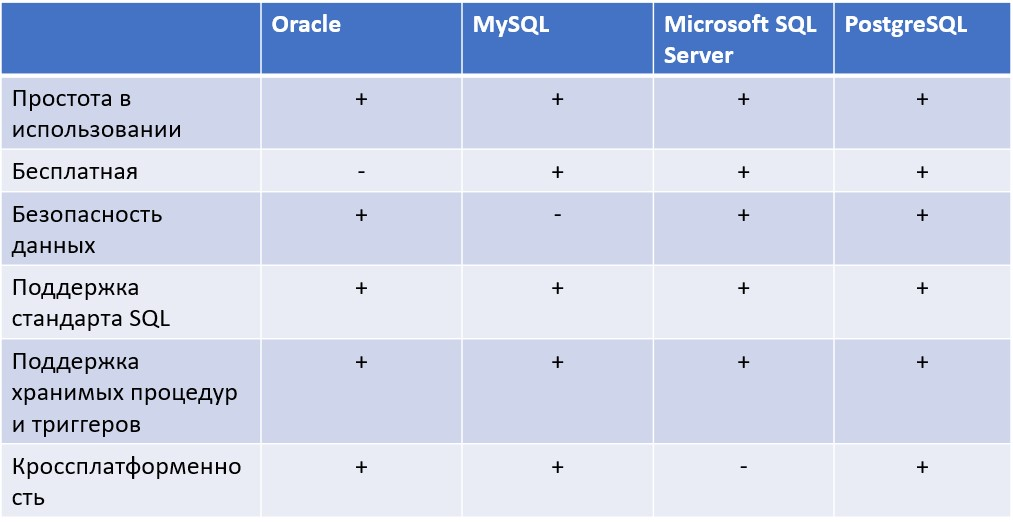
\includegraphics[scale=0.6]{img/subd.jpg}
	\caption{Анализ СУБД.}
	\label{img:subd}
\end{figure}

\subsection{Средства реализации поставленной задачи}
В качестве языка программирования был выбран язык C\#\cite{sharp}, так как:
\begin{itemize}
	\item[1)] этот язык имеет удобные пакеты для работы с PostgreSQL;
	\item[2)] данный язык программирования объектно-ориентирован, что позволит использовать наследование, интерфейсы, абстракции и т.д.
\end{itemize}
В качестве среды разработки была выбрана "Microsoft Visual Studio 2019"\cite{vs}, поскольку:
\begin{itemize}
	\item[1)] она имеет множество удобств для написания и отладки кода;
	\item[2)] является бесплатной для студентов;
	\item[3)] обеспечивает работу с Windows Forms\cite{wf}.  
\end{itemize}
Для данной задачи PostgreSQL\cite{psql} выигрывает по многим параметрам и поэтому было решено использовать именно эту СУБД.

Для работы с базой данных был выбран Entity Framework\cite{efcore}, так как EF Core поддерживает запросы LINQ, отслеживание изменений, обновления и миграции схемы и работает с многими базами данных, включая PostgreSQL.
\subsection{Создание базы данных}
Необходимо построить диаграмму БД по выделенным сущностям. На рисунке \ref{img:DB} представлена диаграмма БД.
\begin{figure}[h!]
	\centering
	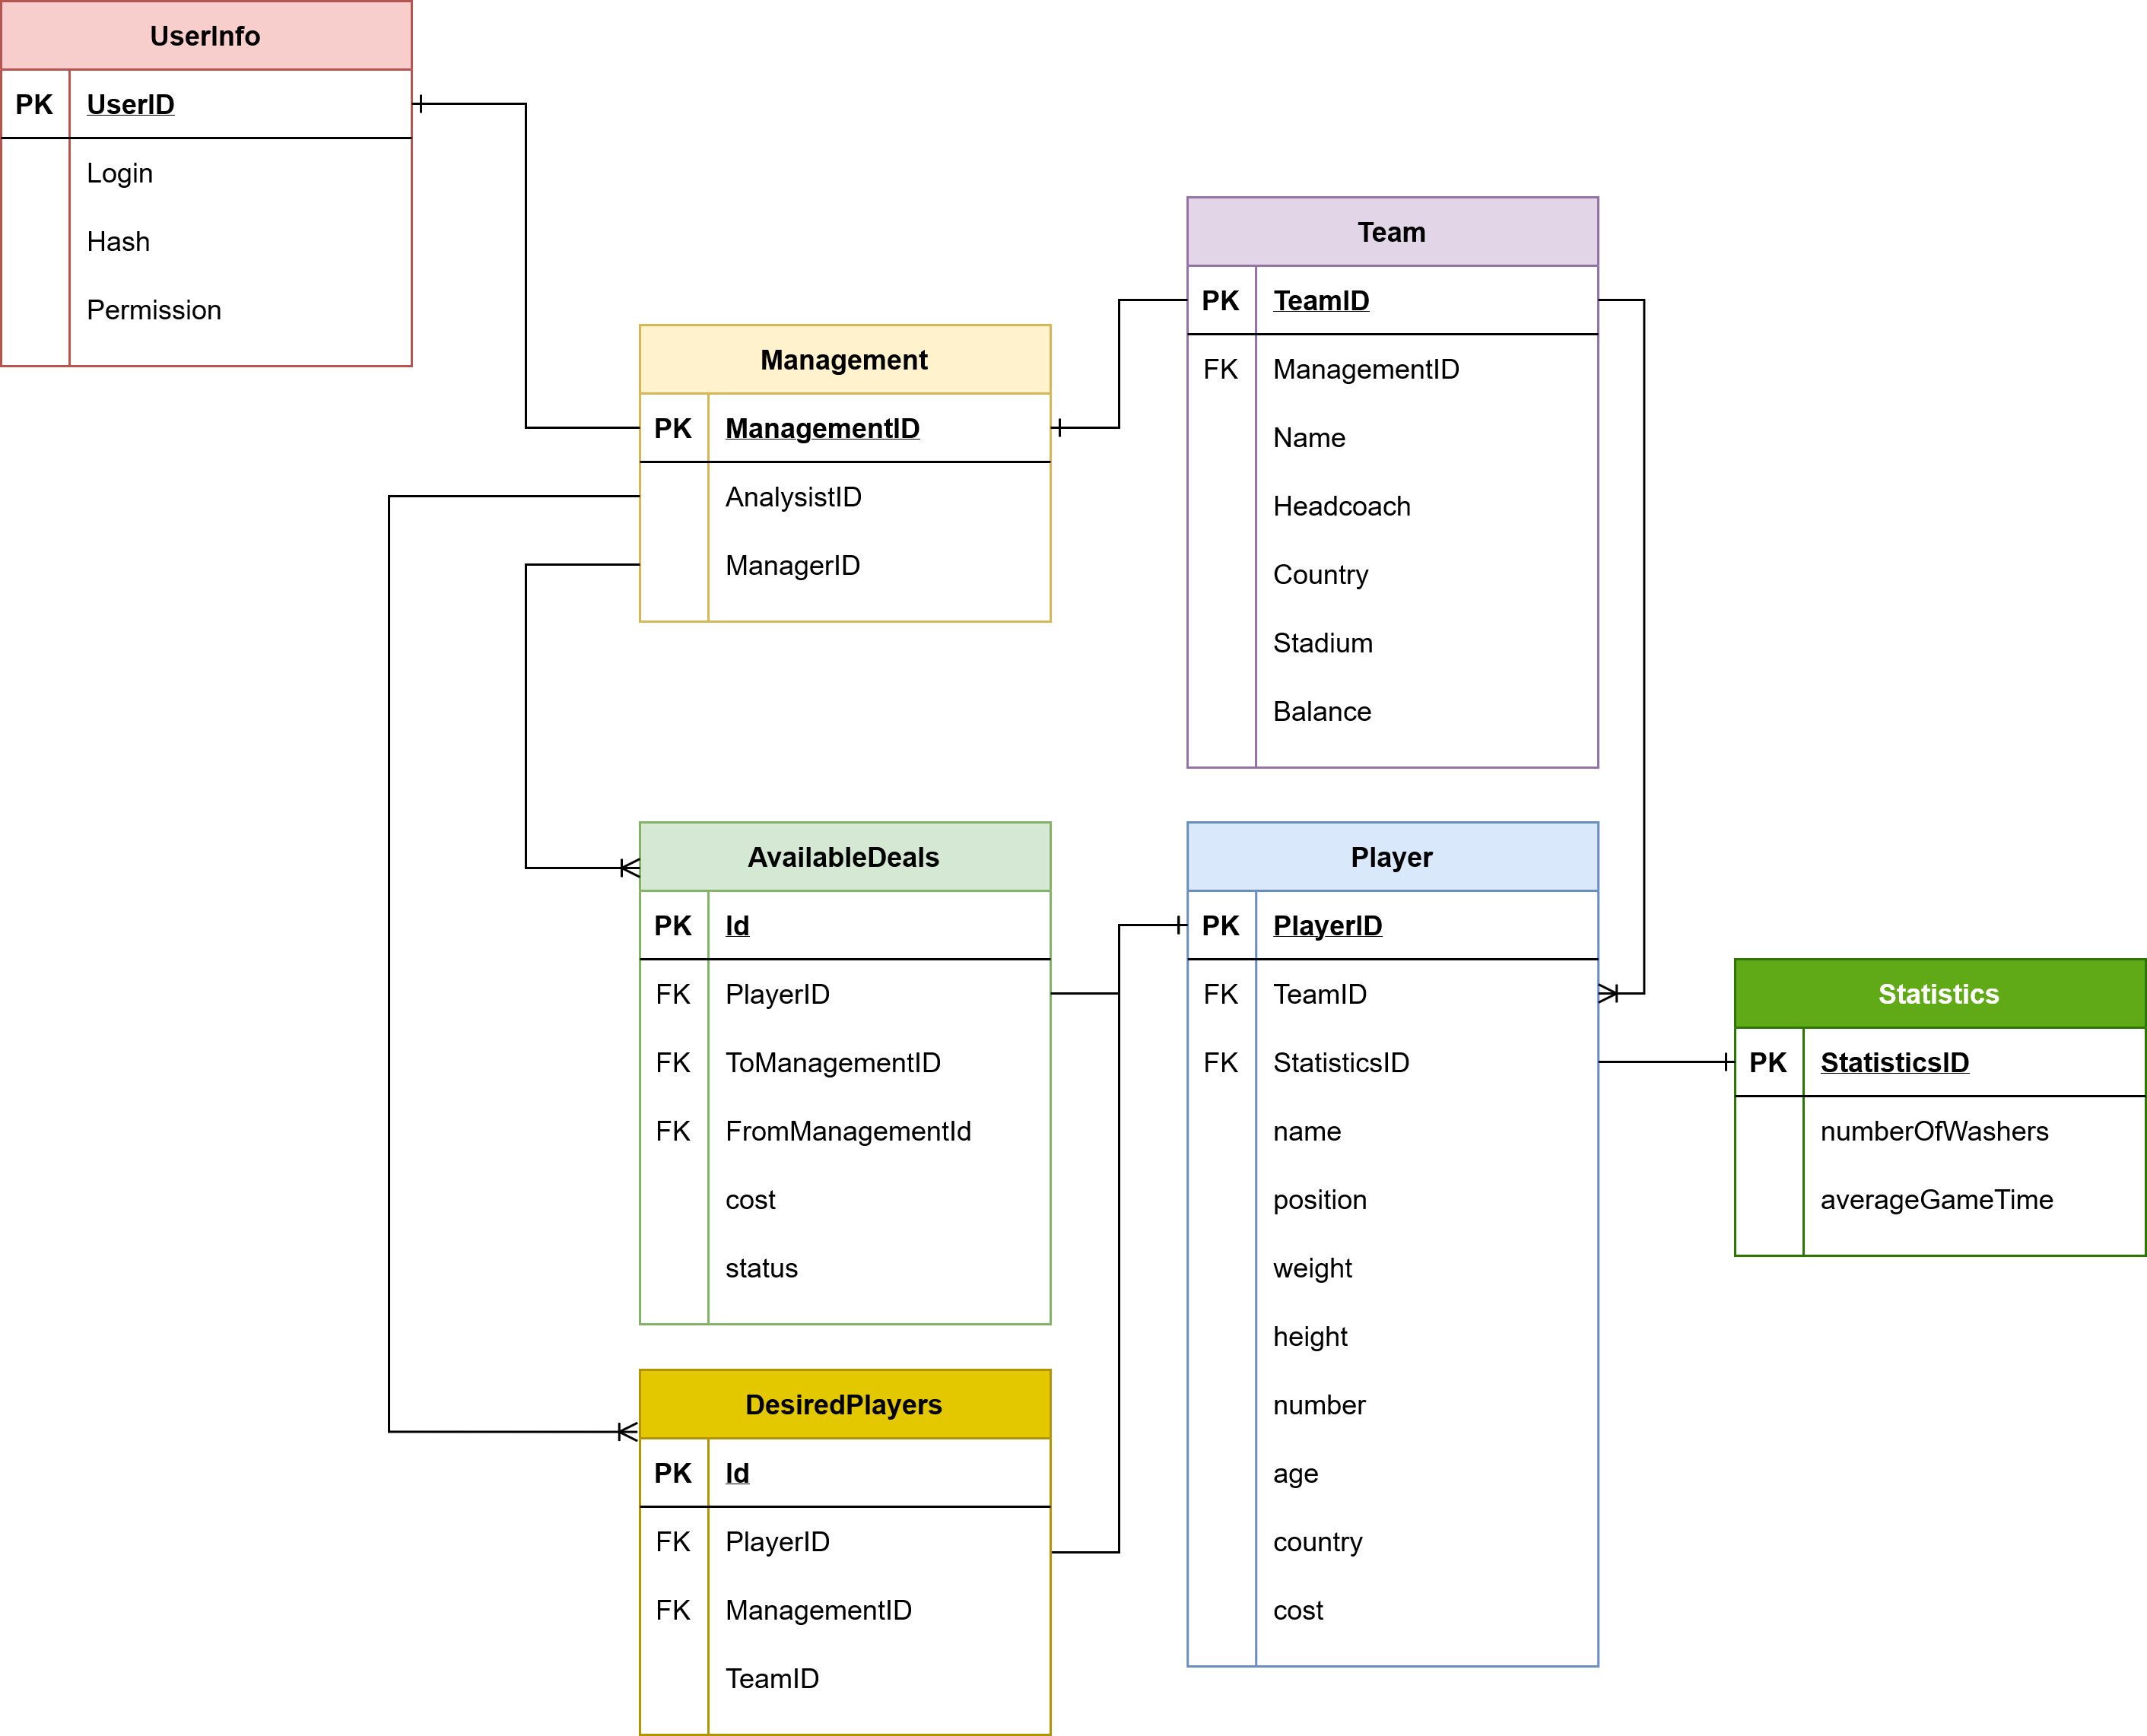
\includegraphics[scale=0.18]{img/DB.png}
	\caption{Диаграмма БД.}
	\label{img:DB}
\end{figure}
\newpage
\subsection{Создание таблиц}
Далее представлены листинги создания таблиц с указанием типов данных каждого столбца.

\textbf{Таблица UserInfo.}
\begin{lstlisting}[label={lst:UserInfo},caption=Создание таблицы UserInfo., language=SQL]
create table if not exists UserInfo (
	id int not null primary key,
	login varchar(30) not null,
	hash varchar(30) not null,
	permission int not null
);
\end{lstlisting}

\textbf{Таблица Management.}
\begin{lstlisting}[label={lst:Manag},caption=Создание таблицы Management., language=SQL]
create table if not exists Management (
	ManagementID int not null primary key,
	AnalysistID int references UserInfo(id),
	ManagerID int references UserInfo(id)
);
\end{lstlisting}

\textbf{Таблица Team.}
\begin{lstlisting}[label={lst:Team},caption=Создание таблицы Management., language=SQL]
create table if not exists Team (
	TeamID int not null primary key,
	ManagementID int references Management(ManagementID),
	Name varchar(30) not null,
	HeadCoach varchar(30) not null,
	Country varchar(30) not null,
	Stadium varchar(60) not null,
	Balance int not null
);
\end{lstlisting}

\textbf{Таблица Player}.
\begin{lstlisting}[label={lst:Player},caption=Создание таблицы Player., language=SQL]
create table if not exists Player (
	PlayerID int not null primary key,
	TeamID int references Team(TeamID),
	Statistics int references Statistics(StatisticsID),
	name varchar(30) not null,
	position varchar(10) not null,
	weight int not null,
	height int not null,
	number int not null,
	age int not null,
	country varchar(50) not null,
	cost int not null
);
\end{lstlisting}

\textbf{Таблица AvailableDeals.}
\begin{lstlisting}[label={lst:AvailableDeals},caption=Создание таблицы AvailableDeals., language=SQL]
create table if not exists AvailableDeals (
	Id int primary key not null,
	PlayerID int references Player(PlayerID),
	ToManagementID int references Management(ManagementID),
	FromManagementID int references Management(ManagementID),
	cost int not null,
	status int not null
);
\end{lstlisting}

\textbf{Таблица DesiredPlayers.}
\begin{lstlisting}[label={lst:DesiredPlayers},caption=Создание таблицы AvailableDeals., language=SQL]
create table if not exists DesiredPlayers (
	Id int primary key not null,
	PlayerID int references Player(PlayerID),
	TeamID int references Team(TeamID),
	ManagementID int references Management(ManagementID)
); 
\end{lstlisting}

\textbf{Таблица Statistics.}
\begin{lstlisting}[label={lst:Statistics},caption=Создание таблицы AvailableDeals., language=SQL]
create table if not exists Statistics (
	StatisticsID int not null primary key,
	numberOfWashers int not null,
	averageGameTime int not null
);
\end{lstlisting}

\subsection{Создание пользователей системы}
Для того, чтобы обеспечить безопасность доступа к данных необходимо создать пользователей с соответствующими правами.

\textbf{Гость}
\begin{lstlisting}[label={lst:guest},caption=Создание пользователя guest., language=SQL]
create role guest with login password '1234';
grant select on table userinfo to guest;
\end{lstlisting}

\textbf{Аналитик}
\begin{lstlisting}[label={lst:analytic},caption=Создание пользователя analytic., language=SQL]
create role analytic with login password '1234';
grant select on table player, team, management, statistics to analytic;
grant all privileges on table desiredplayers to analytic;
\end{lstlisting}

\textbf{Менеджер}
\begin{lstlisting}[label={lst:manager},caption=Создание пользователя manager., language=SQL]
create role manager with login password '1234';
grant select on table player, team, management, statistics to manager;
grant select, delete on table desiredplayers to manager;
grant select, delete, insert on table availabledeals to manager;
\end{lstlisting}

\textbf{Moderator}
\begin{lstlisting}[label={lst:moderator},caption=Создание пользователя moderator., language=SQL]
create role moderator with login password '1234';
grant all privileges on table player, team, management, statistics, availabledeals, desiredplayer, userinfo to moderator;
\end{lstlisting}

\subsection{Функции}
В листинге \ref{lst:func} представлена реализация функции GetPlayers.
\begin{lstlisting}[label={lst:func},caption=Реализация функции GetPlayers., language=SQL]
drop function if exists GetPlayers;
create function GetPlayers()
returns table
(
	PlayerID int,
	Player varchar(40),
	Team varchar(40),
	Washers int,
	gametime int
)
language sql
as $$
	select PlayerTeam.playerid as PlayerID, PlayerTeam.player as Player, 
		PlayerTeam.Team as Team, statistics.numberOfWashers as Washers, 
		statistics.averageGameTime as gametime
	from (
		select PlayerID as playerid, player.Name as player, 
			player.Statistics as PlayerStat, team.Name as Team
		from player join team on player.TeamID = team.TeamID
	) as PlayerTeam
	join statistics on PlayerTeam.PlayerStat = statistics.StatisticsID;
$$;
\end{lstlisting}
Данная функция нужна для того, чтобы получить сразу информацию из нескольких таблиц по игроку. Сначала соединяются таблицы Player и Team по ключу TeamID. Из нее выбираются поля PlayerID, player.Name, player.Statistics, team.Name. В полученной таблице они хранятся под названиями playerid, player, PlayerStat, Team. Ее название - PlayerTeam. Далее полученная таблица соединяется с Statistics по StatisticsID и PlayerStat и из нее выбираются PlayerID, Player, Team, numberOfWashers (Washers), averageGameTime (gametime).

Типы выходных параметров:
\begin{itemize}
	\item[1)] PlayerID - int, так как хранит идентификатор игрока;
	\item[2)] Player - varchar(40), так как хранит имя игрока;
	\item[3)] Team - varchar(40), так как хранит название команды;
	\item[4)] Washers - int, так как хранит количество забитых шайб;
	\item[5)] gametime - int, так как хранит среднее время игры.
\end{itemize}

\subsection{Добавление функции в контекст базы данных}
Так как в программе используется ORM EntityFramework Core, необходимо создать класс, содержащий поля выходных параметров функции.
\begin{lstlisting}[label={lst:table},caption=Класс PlayerTeamStat., language=python]
[Keyless]
public class PlayersTeamStat
{
	public int playerid { get; set; }
	public string player { get; set; }
	public string team { get; set; }
	public int washers { get; set; }
	public int gametime { get; set; }
}
\end{lstlisting}
Keyless обозначает, что данная сущность без ключа.

Далее необходимо создать в классе контекста метод, который проецируется на хранимую функцию и через который можно вызывать данную функцию.
\begin{lstlisting}[label={lst:method},caption=Метод getplayers., language=python]
public IQueryable<PlayersTeamStat> getplayers() => FromExpression(() => getplayers());
\end{lstlisting}
Здесь добавлен метод getplayers(), который соответствует хранимой функции в БД. Он не принимает никакие параметры и возвращает объект IQueryable<PlayersTeamStat>. Этот метод с помощью встроенного в классе DbContext метода FromExpression вызывает getplayers().

Далее в переопрепределенном методе OnModelCreating() класса контекста необходимо зарегестрировать метод getplayers с помощью вызова HasDbFunction():
\begin{lstlisting}[label={lst:registration},caption=Регистрация метода getplayers., language=python]
modelBuilder.HasDbFunction(() => getplayers());
\end{lstlisting}

\subsection{Разработка компонентов}
Так как приложение спроектировано по паттерну MVC, необходимо реализовать компоненты: доступа к данным и бизнес-логики.

\subsubsection{Компонент доступа к данным}
На рисунке \ref{img:AccessToDB} представлена UML-диаграмма компонента доступа к данным.
\begin{figure}[h!]
	\centering
	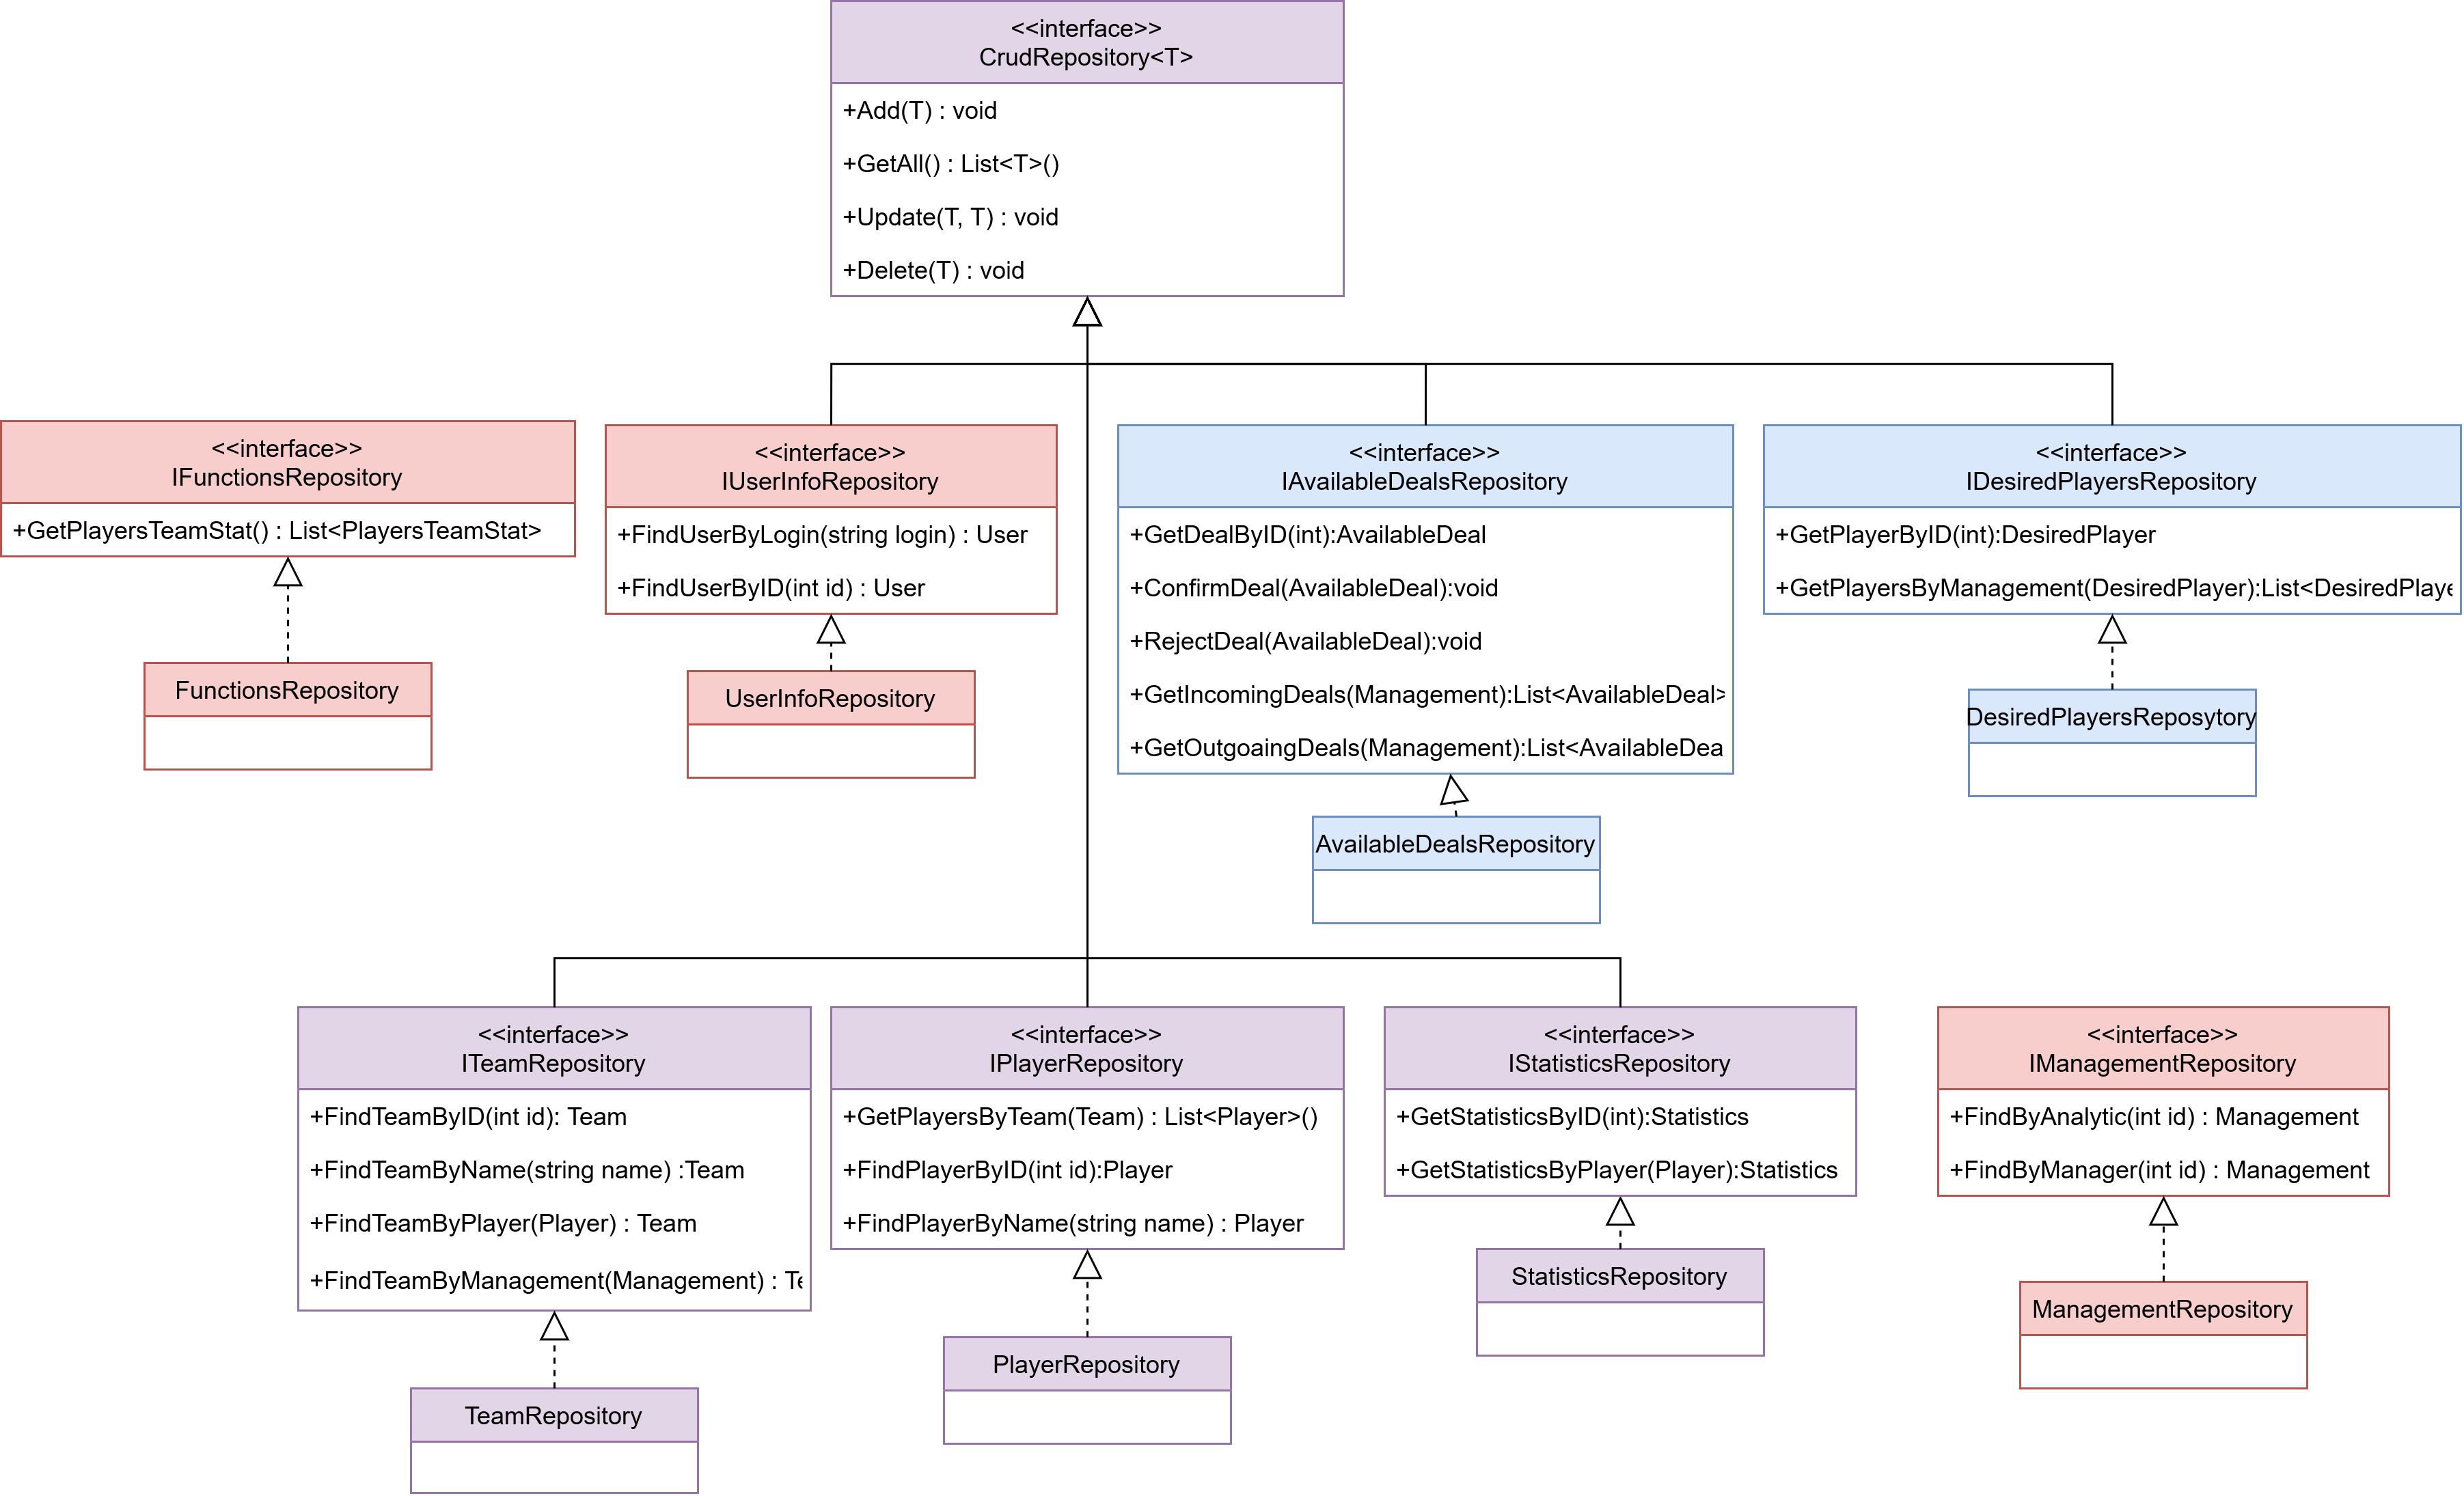
\includegraphics[scale=0.14]{img/AccessToDB.png}
	\caption{Компонент доступа к данным.}
	\label{img:AccessToDB}
\end{figure}
\newpage
\subsubsection{Компонент бизнес-логики}
На рисунке \ref{img:Controllers} представлена UML-диаграмма компонента бизнес-логики.
\begin{figure}[h!]
	\centering
	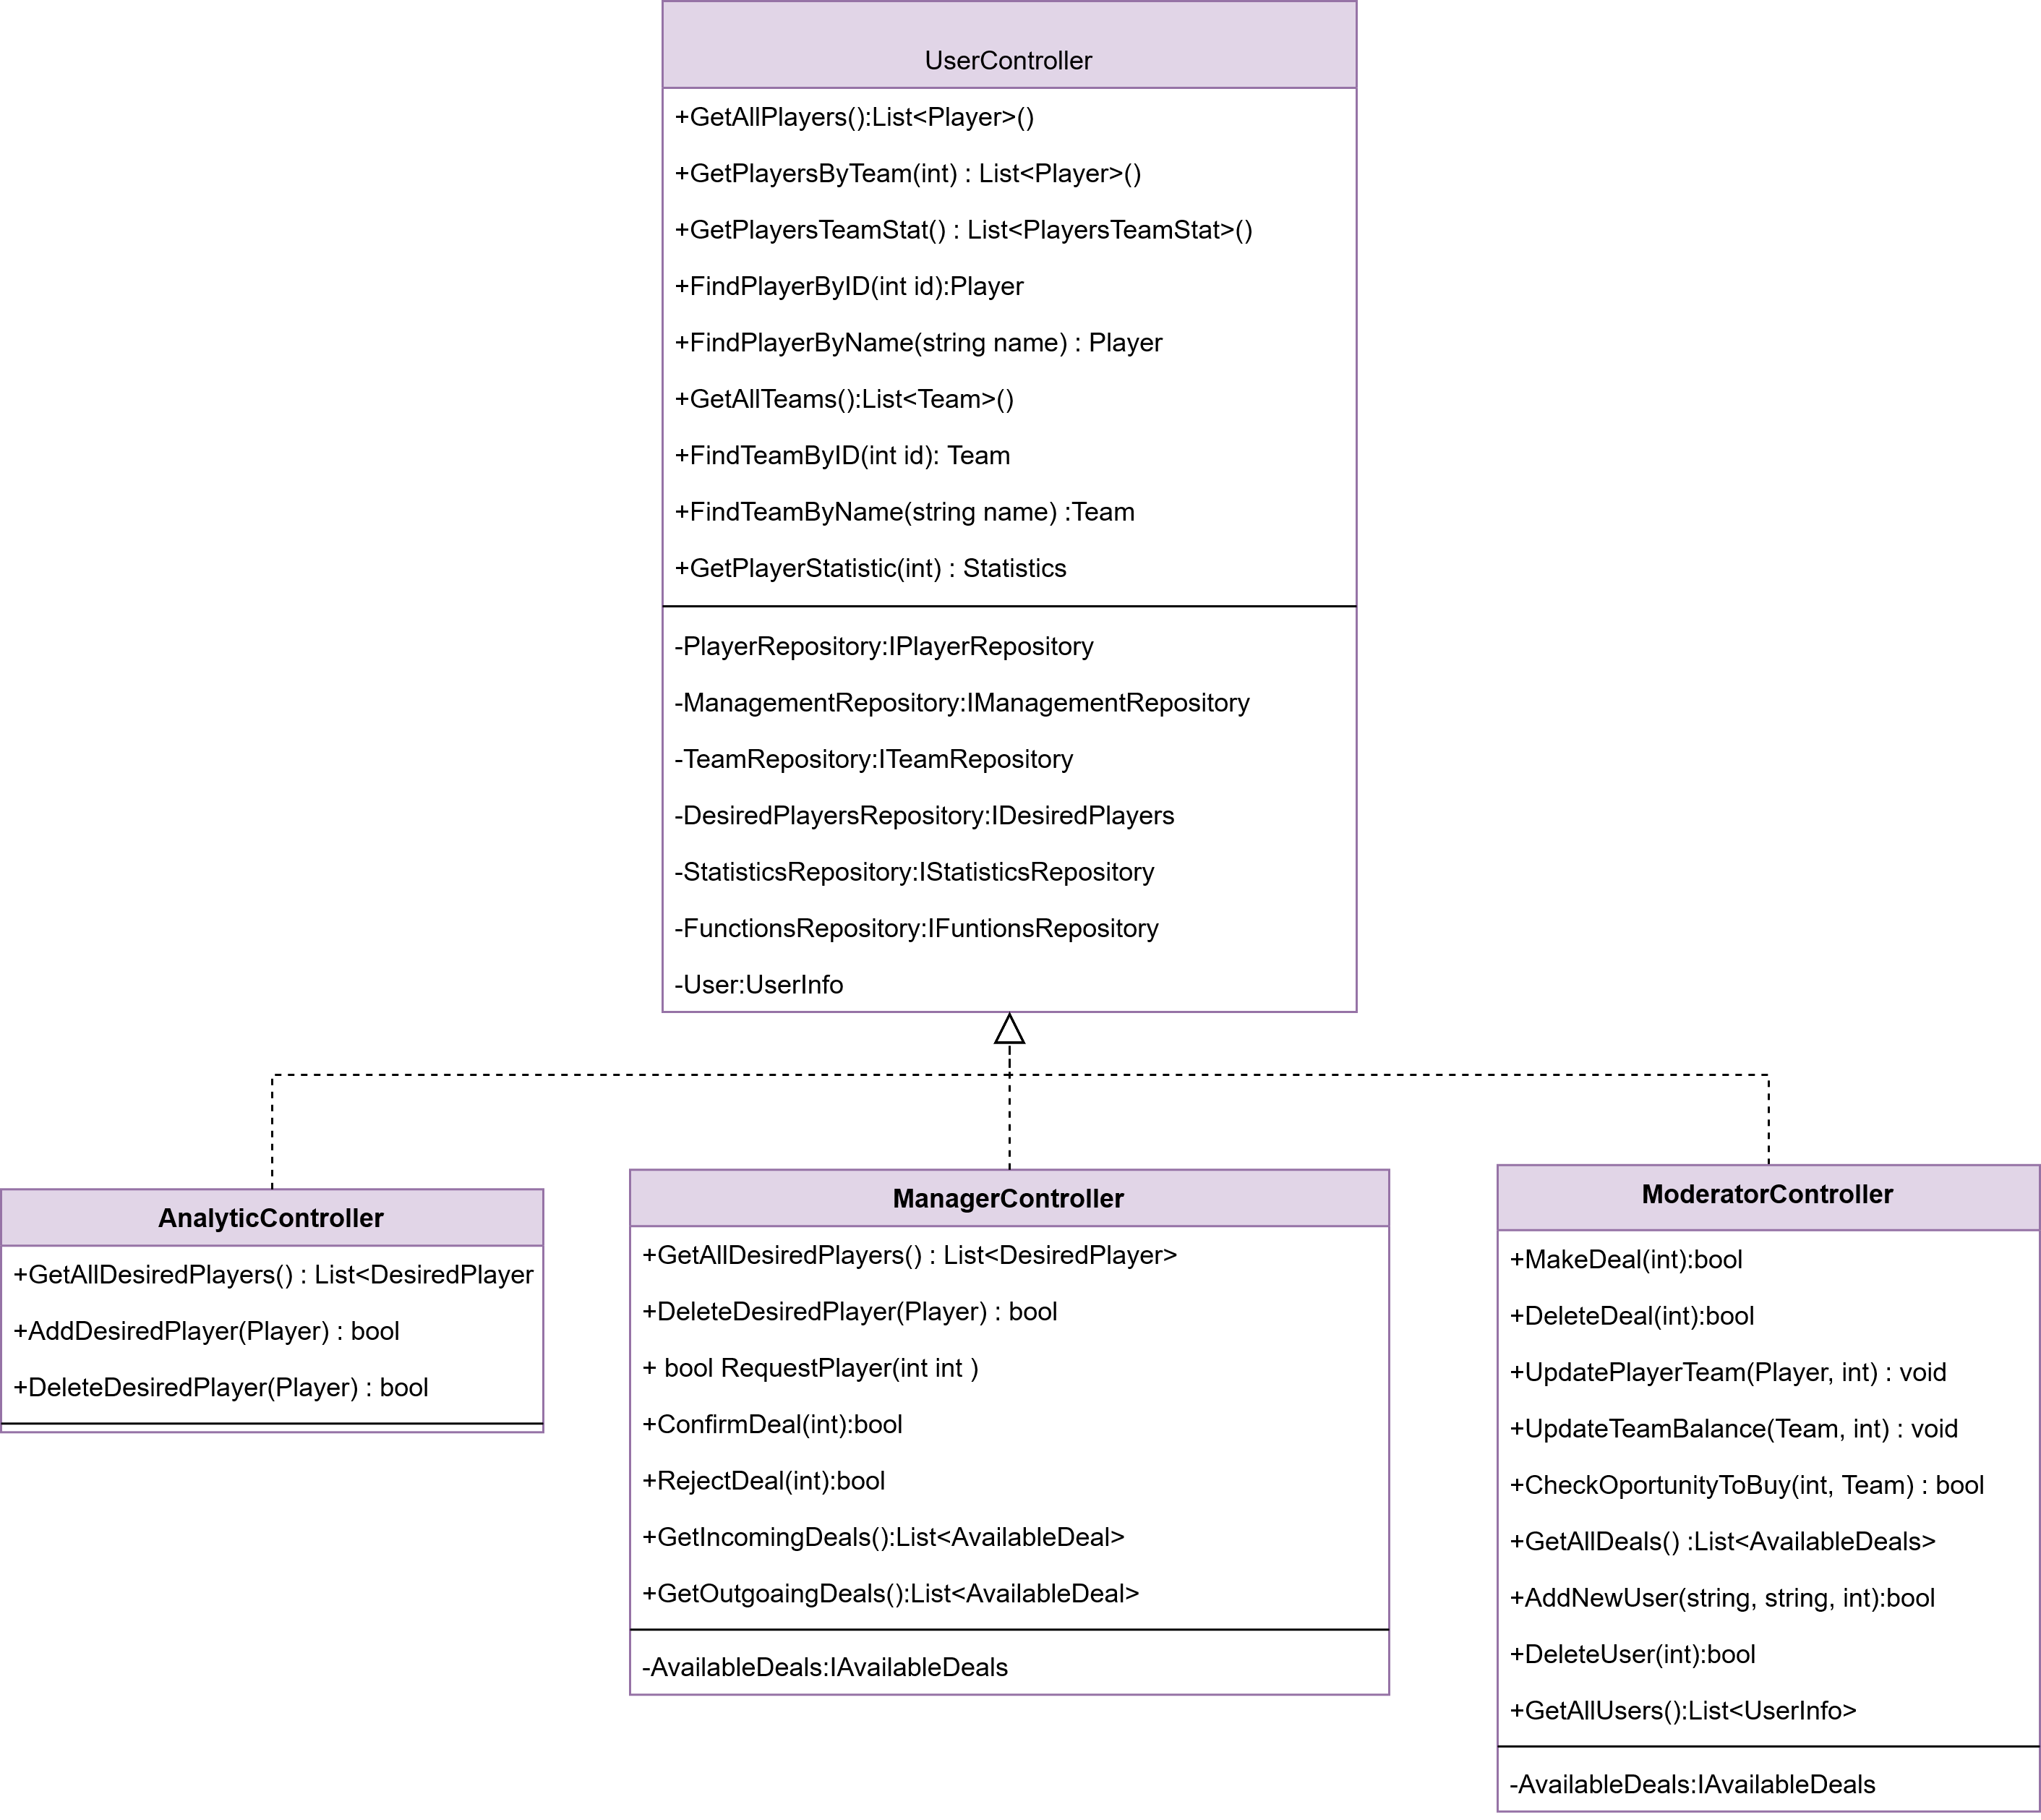
\includegraphics[scale=0.14]{img/Controllers.png}
	\caption{Компонент бизнес-логики.}
	\label{img:Controllers}
\end{figure}
\subsection{Интерфейс приложения}
На рисунках ниже показан интерфейс авторизации и интерфейсы пользователей (аналитик, менеджер, модератор).

На рисунке \ref{img:auth} показана форма авторизации. Для входа в систему пользователю необходимо ввести логин и пароль.
\begin{figure}[h!]
	\centering
	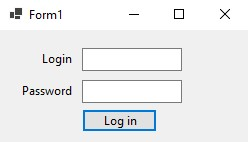
\includegraphics[scale=1]{img/auth.jpg}
	\caption{Окно авторизации.}
	\label{img:auth}
\end{figure}
\newpage
На рисунке \ref{img:main} показан основной интерфейс пользователя. Всего 4 группы: команды доступные любому пользователю и команды аналитика, менеджера и модератора. Также выведена информация о текущем пользователе (логин, пароль, права доступа и идентификатор).
\begin{figure}[h!]
	\centering
	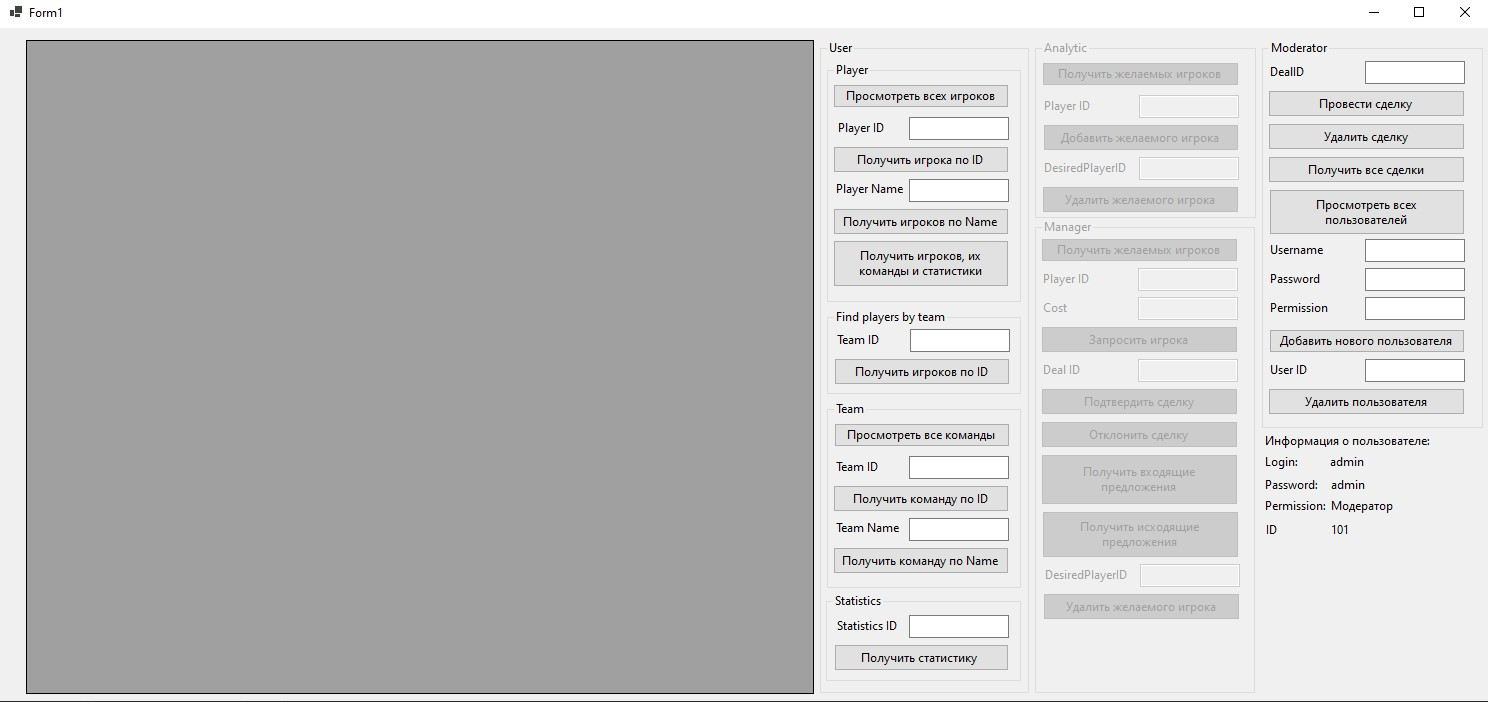
\includegraphics[scale=0.4]{img/main.jpg}
	\caption{Основное окно.}
	\label{img:main}
\end{figure}
\clearpage
На рисунке \ref{img:analytic} показаны команды, доступные аналитику. Любой аналитик может просмотреть желаемых игроков, а также удалить и добавить нового. Функции менеджера и модератора для него недоступны.
\begin{figure}[h!]
	\centering
	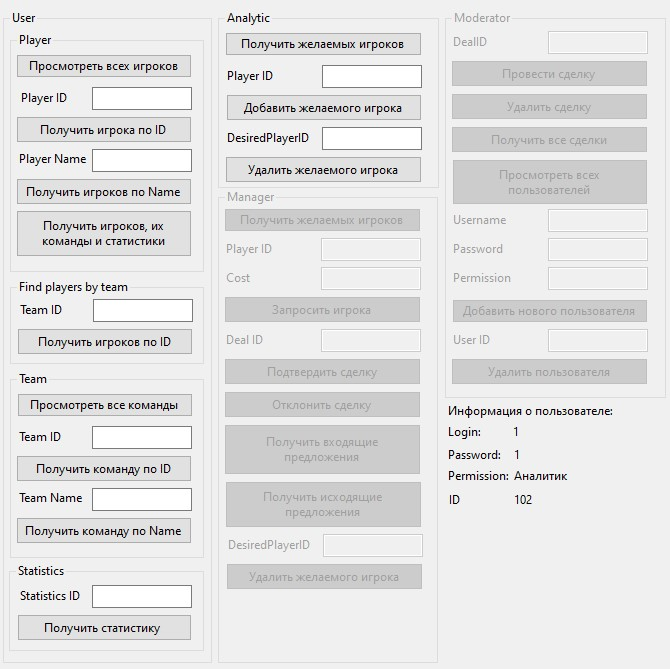
\includegraphics[scale=0.90]{img/analytic.jpg}
	\caption{Операции, доступные аналитику.}
	\label{img:analytic}
\end{figure}
\clearpage
На рисунке \ref{img:manager} показаны команды, доступные менеджеру. Любой менеджер может просмотреть желаемых игроков, а также удалить ненужного, также может запрашивать игрока на покупку, проводить и отклонять сделки и получить входящие и исходящие предложения. Функции аналитика и модератора для него недоступны.
\begin{figure}[h!]
	\centering
	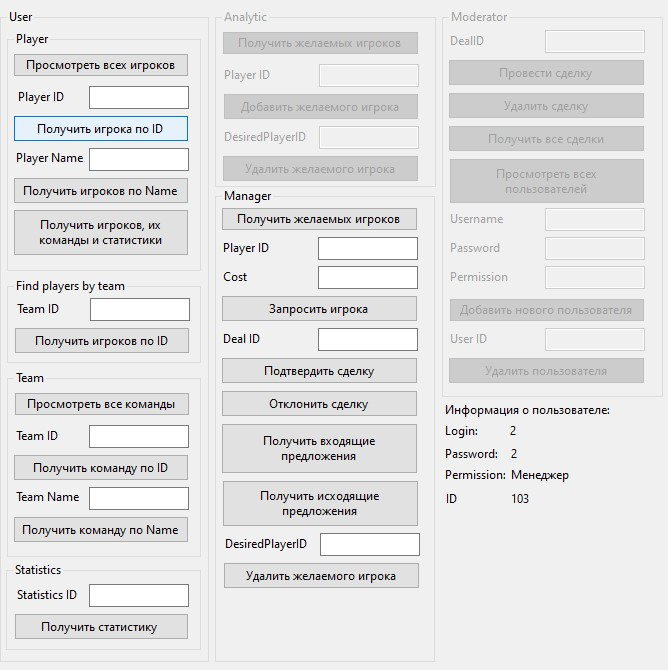
\includegraphics[scale=0.90]{img/manager.jpg}
	\caption{Операции, доступные менеджеру.}
	\label{img:manager}
\end{figure}
\clearpage
На рисунке \ref{img:moderator} показаны команды, доступные модератору. Любой модератор может получить, провести и удалить сделки, добавить, удалить и просмотреть пользователей. Функции аналитика и менеджера для него недоступны.
\begin{figure}[h!]
	\centering
	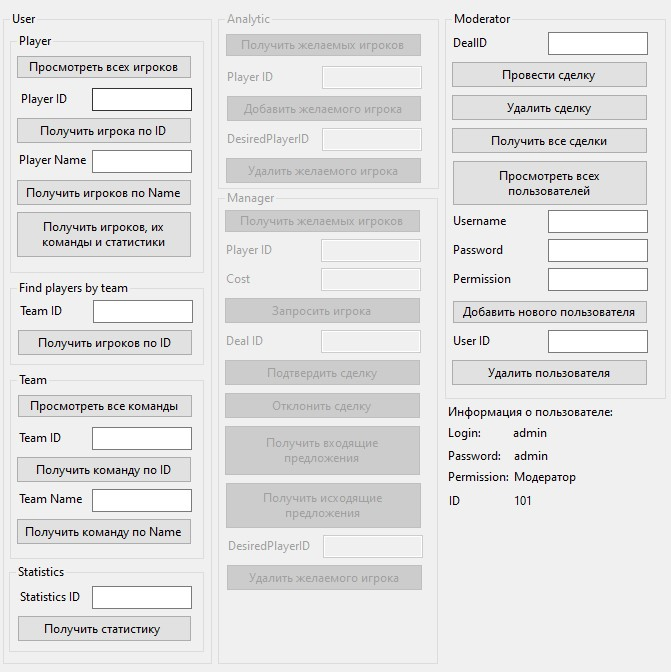
\includegraphics[scale=0.90]{img/moderator.jpg}
	\caption{Операции, доступные модератору.}
	\label{img:moderator}
\end{figure}

\subsection{Вывод}
В данном разделе были выбраны средства реализации поставленной задачи, создана база данных и описана ролевая модель на уровне БД, разработаны компоненты и описан порядок работы.
\newpage
\section*{Заключение}
\addcontentsline{toc}{section}{Заключение}
Цель курсовой работы достигнута.

В ходе выполнения курсовой работы было формализовано задание, выделены соответсвующие пользователи и их функционал, проведен анализ СУБД и выбрана наиболее подходящая для данной задачи, спроектирована база данных, архитектура приложение.

В результате, с использованием языка программирования C\# и СУБД PostgreSQL было создано многофункциональное приложение для получения информации об игроках с возможностью их покупки и продажи. Получен опыт разработки базы данных и приложения по паттерну MVC. 

В дальнейшей перспективе приложение и база данных могут был масштабированы. Может быть добавлен следующий функционал:
\begin{itemize}
	\item[1)] возможность добавления модератором игроков и команд;
	\item[2)] возможность добавления нескольких лиг для команд и перехода игроков по лигам;
	\item[3)] могут быть добавлены другие пользователи, например игрок, менеджер игрока и т.д.
\end{itemize}

\clearpage
%СПИСОК ЛИТЕРАТУРЫ
\begin{thebibliography}{9}
	\addcontentsline{toc}{section}{Литература}
	\bibitem{sharp} Документация по C\# [Электронный ресурс] URL: https://docs.microsoft.com/ru-ru/dotnet/csharp/ (дата обращения: 20.05.2021).
	\bibitem{vs} Документация по семейству продуктов Visual Studio [Электронный ресурс] URL: https://docs.microsoft.com/ru-ru/visualstudio/?view=vs-2019 (дата обращения: 20.05.2021).
	\bibitem{wf} Windows Forms [Электронный ресурс] URL: https://docs.microsoft.com/ru-ru/dotnet/desktop/winforms/?view=netdesktop-5.0 (дата обращения: 20.05.2021).
	\bibitem{psql} PostgreSQL : Документация [Электронный ресурс] URL: https://postgrespro.ru/docs/postgresql (дата обращения: 20.05.2021).
	\bibitem{efcore} Документация по Entity Framework [Электронный ресурс] URL: https://docs.microsoft.com/ru-ru/ef/ (дата обращения: 20.05.2021).
\end{thebibliography}

\addcontentsline{toc}{section}{Приложение А. Презентация.}

\end{document}
